%\documentclass{standalone}
%\usepackage{tikz}

%% The general formula of projection of point (x_1,x_2,x_3) is $P(x_1,x_2,x_3)=(-\sqrt{3}/2*(x_1-x_2) , -(1/2)*x_{1} - (1/2)*x_{2} + x_{3})$.

\def\coord#1#2#3{{-sqrt(3)/2*(#1-#2)} ,{ -(1/2)*#1 - (1/2)*#2 + #3}}
%\begin{document}
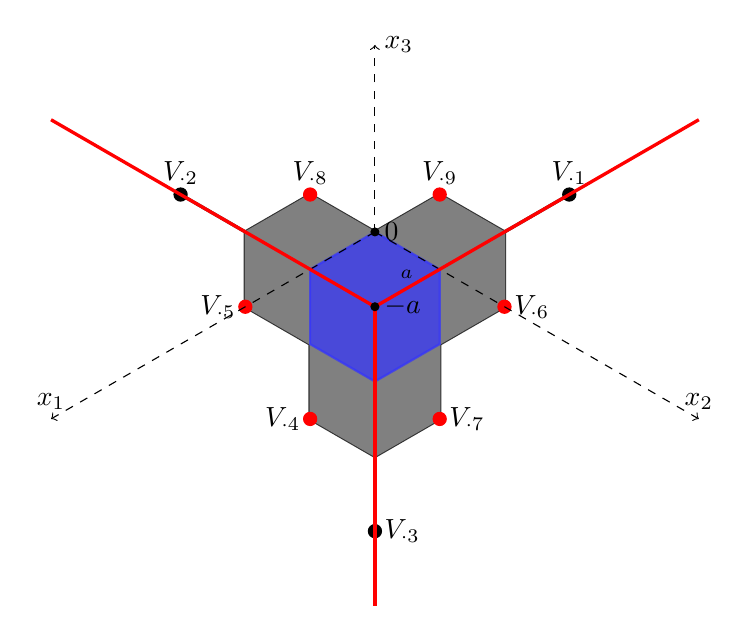
\begin{tikzpicture}[scale=0.95]

\coordinate (v1) at (\coord{-3}{0}{-1});
\coordinate (v2) at (\coord{0}{-3}{-1});
\coordinate (v3) at (\coord{0}{0}{-4});
\coordinate (v4) at (\coord{1}{0}{-2});
\coordinate (v5) at (\coord{1}{-1}{-1});
\coordinate (v6) at (\coord{-1}{1}{-1});
\coordinate (v7) at (\coord{0}{1}{-2});
\coordinate (v8) at (\coord{0}{-1}{0});
\coordinate (v9) at (\coord{-1}{0}{0});

\coordinate (v1p) at (\coord{-5}{0}{-1});
\coordinate (v2p) at (\coord{0}{-5}{-1});
\coordinate (v3p) at (\coord{0}{0}{-5});

\coordinate (f1) at (\coord{-2}{0}{-1});
\coordinate (f2) at (\coord{0}{-2}{-1});
\coordinate (f3) at (\coord{0}{0}{-3});

\coordinate (b1) at (\coord{0}{0}{0});
\coordinate (b2) at (\coord{0}{1}{0});
\coordinate (b3) at (\coord{0}{1}{-1});
\coordinate (b4) at (\coord{0}{0}{-2});
\coordinate (b5) at (\coord{1}{0}{-1});
\coordinate (b6) at (\coord{1}{0}{0});

%% \fill[red!30,opacity=0.7] (v1p) -- (\coord{0}{0}{-1}) -- (v2p)--cycle;
%% \fill[blue!30,opacity=0.7] (v1p) -- (\coord{0}{0}{-1}) -- (v3p)--cycle;
%% \fill[green!30,opacity=0.7] (v2p) -- (\coord{0}{0}{-1}) -- (v3p)--cycle;


\filldraw[black,draw=black,opacity=0.8,very thick] (v1) -- (f1) -- (v9) -- (b1) -- (v8) -- (f2) -- (v2) -- (f2) -- (v5) -- (b5) -- (v4) -- (f3) -- (v3) -- (f3) -- (v7) -- (b3) -- (v6) -- (f1) -- (v1) -- cycle;
\filldraw[gray] (f1) -- (v9) -- (b1) -- (v8) -- (f2) -- (v5) -- (b5) -- (v4) -- (f3) -- (v7) -- (b3) -- (v6) -- (f1) -- cycle;

\filldraw[blue!80,draw=blue!80,opacity=0.7, thick] (b1) -- (b2) -- (b3) -- (b4) -- (b5) -- (b6) -- (b1) -- cycle;


\filldraw[black] (v1) circle (2.5pt) node[above] {$V_{\cdot 1}$};
\filldraw[black] (v2) circle (2.5pt) node[above] {$V_{\cdot 2}$};
\filldraw[black] (v3) circle (2.5pt) node[below,right]{$V_{\cdot 3}$};
\filldraw[red] (v4) circle (2.5pt) node[below,left,black] {$V_{\cdot 4}$};
\filldraw[red] (v5) circle (2.5pt) node[below,left,black] {$V_{\cdot 5}$};
\filldraw[red] (v6) circle (2.5pt) node[below,right,black] {$V_{\cdot 6}$};
\filldraw[red] (v7) circle (2.5pt) node[below,right,black] {$V_{\cdot 7}$};
\filldraw[red] (v8) circle (2.5pt) node[above,black] {$V_{\cdot 8}$};
\filldraw[red] (v9) circle (2.5pt) node[above,black] {$V_{\cdot 9}$};

\draw[dashed,->] (\coord{0}{0}{0}) -- (\coord{5}{0}{0}) node[above] {$x_1$};
\draw[dashed,->] (\coord{0}{0}{0}) -- (\coord{0}{5}{0}) node[above] {$x_2$};
\draw[dashed,->] (\coord{0}{0}{0}) -- (\coord{0}{0}{2.5}) node[above, right] {$x_3$};
\filldraw[black] (\coord{0}{0}{0}) circle (1.5pt) node[below,right] {0};

%The regression hyperplane
\draw[very thick,red] (\coord{0}{0}{-1}) -- (v1p);
\draw[very thick,red] (\coord{0}{0}{-1}) -- (v2p);
\draw[very thick,red] (\coord{0}{0}{-1}) -- (v3p);
\filldraw[black] (\coord{0}{0}{-1}) circle (1.5pt) node[below,right] {$-a$};
\draw node[above] at (\coord{-1/2}{0}{-1}) {$\cH_a$};


\end{tikzpicture}
%\end{document}




